\section{Durchführung und Aufbau}
\label{sec:Durchführung}
Um das Trägheitsmoment verschiedener Objekte $I_O$ zu bestimmen, werden diese an einer Drillachse fixiert und deren Schwingungsdauern gemessen. Die Drillachse besteht aus einem Rahmen, woran eine Torsionsfeder befestigt ist. Diese ist des weiteren mit einer Achse verbunden, wo verschdieden Testobjekte eingespannt werden können, wie in Abbildung \ref{fig:drillachse} zu sehen ist. 
\ \\
\begin{figure}[ht]
	\centering
	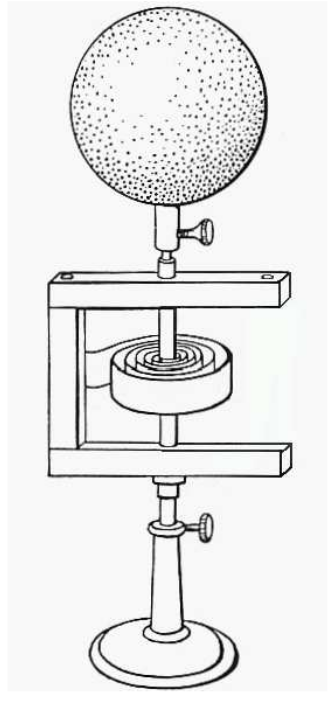
\includegraphics[height=4.5cm]{Abbildung1.png}
	\caption{Versuchsaufbau\cite{sample}}
	\label{fig:drillachse}
\end{figure}

Um zunächst die Winkelrichtgöße $D$ der Drillasches zu bestimmen, wird ein nahezu masseloser Stab an der Drillachse befestigt und mittels einer Federwaage die benötigte Kraft für die  Auslenkung aus der Ruheposition gemessen. Aus der Proportionalität der Kraft mit dem Winkel soll $D$ bestimmt werden. 
\\
\\
Nachdem die Winkelrichtgröße mittels einer statischen Methode bestimmt wurde soll nun das Eigenträgheitsmoment der Drillachse bestimmt werden. Dazu wird an der Achse einen nahezu masseloser Stab befestigt, an welchem im Abstand $r$ zur Drehachse Gewichte fixiert werden. Nun wird der Stab ausgelenkt und die fünffache Schwingungsdauer gemessen. Aus der Schwingungsdauer und der Kenntnis des Trägheitsmoments der fixierten Gewichtes und des Stabes, lässt sich das Trägheitsmoment der Drillachse $I_D$ bestimmen.
\\
\\
Anschließend soll das Trägheitsmoment zweier Körper bestimmt werden. Dazu wird die Masse und das Volumen der Körper bestimmt, um sie später mit dem theoretischen Trägheitsmomenten vergleichen zu können. Als nächstes wird der Körper auf der Drillachse befestigt und ausgelenkt um, eine Schwingung zu erzeugen. Es werden 5 Schwingungsdauern je 5 mal gemessen und die Werte anschließend gemittelt. 
\\
\\
Zur bestimmung des Trägheitsmoment einer Puppe wird diese an der Drillachse befestigt. Es werden zwei verschieden Position der Puppe gewählt und deren Schwingungsdauer bestimmt. Desweiteren muss die Puppe in geeignete mathematische Körper zerlegt werden und dessen Abmaße bestimmt werden um die einzelen Trägheitsmomente der verschiedenen Körperteile zu errechnen. Die Summe aus den verschieden Körperteilen entspricht dann dem Trägheitsmoment der gesamten Puppe.
